\documentclass[a4paper]{article}

\usepackage{times}
\usepackage{tikz}
\usepackage[margin=0cm]{geometry}
\usepackage{graphicx}
\usepackage{anyfontsize}
\usepackage{fancyhdr}
\usepackage{indentfirst}
\usepackage{amsmath}
\usepackage[spanish]{babel}
\usepackage[utf8]{inputenc}
\usepackage{titlesec}
\usepackage{enumitem}
\usepackage{caption}
\usepackage{booktabs}

\author{}
\date{}
\title{}


\begin{document}
\thispagestyle{empty}

\newcommand{\saltoPag}{\newpage \noindent \thispagestyle{fancy}}

\begin{tikzpicture}[remember picture, overlay]
    \pgftransformshift{\pgfpoint{0cm}{0cm}}
    \draw [line width=2pt](1cm,-1cm) -- (1cm,-27.7cm) -- (14cm, -27.7cm) -- (14cm, -1cm) -- (1cm, -1cm);
    \draw[line width=2pt] (15cm, -27.7cm) -- (19cm,-27.7cm) -- (19cm, -1cm) -- (15cm, -1cm) --  (15cm, -27.7cm);
    \node [line width=2pt] at (17cm, -3.5cm) {
\includegraphics[width=3cm]{../../imagenes/utn.png}};
		\node [line width=2pt] at (7.5cm, -7.5cm) {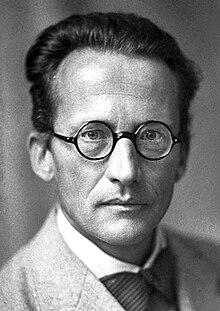
\includegraphics[width=6cm]{../../imagenes/schrodinger.jpeg}};
    \node at (17cm, -7cm) {\scalebox{5}{\textbf{U}}};
    \node at (17cm, -9cm) {\scalebox{5}{\textbf{T}}};
    \node at (17cm, -11cm) {\scalebox{5}{\textbf{N}}};
    \node at (17cm, -14cm) {\scalebox{5}{\textbf{F}}};
    \node at (17cm, -16cm) {\scalebox{5}{\textbf{R}}};
    \node at (17cm, -18cm) {\scalebox{5}{\textbf{C}}};
    \node at (7.4cm, -13cm) {\scalebox{2.5}{\textbf{Ecuación}}};
    \node at (7.4cm, -14cm) {\scalebox{2.5}{\textbf{de}}};
    \node at (7.4cm, -15cm) {\scalebox{2.5}{\textbf{Shrödinger}}};

    \node at (7.5cm, -22cm) {
        \begin{minipage}[c]{12cm}
            \begin{itemize}
                \raggedright
                \vspace{1.5cm}
                \item \fontsize{12}{12}\selectfont \textbf{Autores:} \vspace {1mm} \fontsize{11}{12}\selectfont \\
                    \begin{itemize}
                        \item \hspace{2mm} Valentino Rao - Leg. 402308 \\
                        \item \hspace{2mm} Ignacio Ismael Perea - Leg. 406265 \\
                        \item \hspace{2mm} Manuel Leon Parfait - Leg. 406599 \\ 
                        \item \hspace{2mm} Gonzalo Filsinger - Leg. 400460 \\ 
                        \item \hspace{2mm} Agustín Coronel - Leg. 402010 \\
                        \item \hspace{2mm} Santiago Pannunzio - Leg. 402350 \\
                        \item \hspace{2mm} Marcos Raúl Gatica - Leg. 402006 \\
                    \end{itemize}

                \item \fontsize{12}{12}\selectfont \textbf{Curso:} 2R1. \\
                \item \fontsize{12}{12}\selectfont \textbf{Asignatura:} Física electrónica. \\
                \item \fontsize{12}{12}\selectfont \textbf{Institución:} Universidad Tecnológica Nacional - Facultad Regional de Córdoba \\

            \end{itemize}
        \end{minipage}};

\end{tikzpicture}

\renewcommand{\normalsize}{\fontsize{12}{18}\selectfont}
\newgeometry{margin=2.54cm} %Quiero dejar esto cercano a las normas APA
\fancyhf{}
\renewcommand{\headrulewidth}{0pt}
\renewcommand{\footrulewidth}{0.4pt}
\fancyfoot[R]{[Rao V. - Parfait M. - Filsinger G. - Perea I. - Coronel A - Gatica M.] [\textbf{pág. \thepage}]}
\setlength{\footskip}{1.5cm}
\newpage
\thispagestyle{empty}
\text{}

\titleformat{\section} {\fontsize{12}{12}\bfseries}{\thesection.}{0.5em}{\underline}

\newpage
\newpage

\thispagestyle{empty}
\setcounter{page}{0}
\tableofcontents

\saltoPag
\twocolumn
\flushbottom

\section{Forma de estado estacionario}
        \subsection{Desarrollo}

        \indent En muchas situaciones, la energía potencial de una partícula no depende explícitamente del tiempo; las fuerzas que actúan sobre ella, y por lo tanto $U$, varían solo con la posición de la partícula. Cuando esto es cierto, la ecuación de Schrödinger puede simplificarse eliminando toda referencia a $t$.
        Comenzamos observando que la función de onda unidimensional de una partícula no restringida puede escribirse como:

            \begin{align*}
            \Psi &= Ae^{-j \cdot (\hbar^{-1}) \cdot (Et-px)} \\
            \Psi &= A e^{-jEt \cdot \hbar^{-1}} \cdot e^{jpx \cdot \hbar^{-1}} \\
            \Psi &= \psi(x) e^{-jEt/\hbar}
            \end{align*}

        \indent Donde $\Psi$ es el producto de una función dependiente del tiempo $e^{-jEt \cdot \hbar^{-1}}$ y de una función dependiente de la posición $\psi$. Si sustituimos $\Psi$ en la ecuación de Schrödinger dependiente del tiempo, obtenemos:

            \begin{equation}
            E \cdot \psi e^{-tjE \cdot \hbar^{-1}} = -\frac{\hbar^2}{2m} \cdot e^{-tjE \cdot \hbar^{-1}} \cdot \frac{\partial^2 \psi}{\partial x^2} + U \cdot \psi e^{-tjE \cdot \hbar^{-1}} \\
            \end{equation}

        \indent Si despejamos $\frac{\partial^2 \psi}{\partial x^2}$, obtenemos:

        \begin{align*}
            &E \cdot \psi - U \cdot \psi = -\frac{\hbar^2}{2m} \cdot \frac{\partial^2 \psi}{\partial x^2} \\
            &(E - U) \psi \cdot \frac{2m}{\hbar^2} = -\frac{\partial^2 \psi}{\partial x^2} \\
            &(E - U) \psi \cdot \frac{2m}{\hbar^2} - \frac{\partial^2 \psi}{\partial x^2} = 0
        \end{align*}

        \indent Esta es la ecuación de Schrödinger independiente del tiempo para una partícula no restringida en una sola dimención. La solución de esta ecuación es una función de onda $\psi$ que depende solo de la posición y que satisface la condición de que la energía total de la partícula es igual a la suma de su energía cinética y su energía potencial. La ecuación de Schrödinger independiente del tiempo es una ecuación diferencial de segundo orden que puede resolverse para obtener la función de onda $\psi$.
        \indent Una propiedad importante de la ecuación de estado estacionario de Schrödinger es que, si tiene una o más soluciones para un sistema dado, cada una de estas funciones de onda corresponde a un valor específico de la energía E. Así, la cuantización de la energía aparece en la mecánica ondulatoria como un elemento natural de la teoría, y la cuantización de la energía en el mundo físico se revela como un fenómeno universal característico de todos los sistemas estables.

    \newpage
    \noindent
    \thispagestyle{fancy}
        
    \section{Valores propios y Funciones propias}

    \indent Los valores $E_n$ para los cuales la ecuación de Schrödinger tiene soluciones no triviales se llaman valores propios de la ecuación. Las funciones de onda correspondientes a estos valores propios se llaman funciones propias. Por ejemplo los valores propios para los niveles de energía discreta del átomo de hidrógeno son:

    \begin{align*}
        E_n &= -\frac{m_e e^4}{32 \pi^2 \epsilon_0^2 \hbar^2 n^2} \\
    \end{align*}

    \indent Donde $n$ es un número entero positivo y $m_e$ es la masa del electrón. 

    \indent Una variable dinámica G puede no estar cuantizada. En este caso, las mediciones de $G$ realizadas en varios sistemas idénticos no producirán un resultado único, sino una dispersión de valores cuyo promedio es el valor esperado.La condición para que una cierta variable dinámica $G$ esté restringida a los valores discretos $G_n$,en otras palabras, que G esté cuantizada,es que las funciones de onda $\ \psi_n$ del sistema sean tales que

    \begin{minipage}[c]{7.5cm}

        \vspace{0.5cm}
        \centering
        \textbf{Ecuaciones de valores propios}
        \vspace{-5mm}

        \begin{align*}
            \hat{G} \psi_n = G_n \psi_n
        \end{align*}
    \end{minipage}

    \section{Partícula en una caja}

        \subsection{Pozo de potencial infinito}

        \indent Como las condiciones limites y la normalización determinan las funciones de onda.\\
        \indent Para resolver la ecuación de Schrödinger, incluso en su estado estacionario, es necesario conocer las condiciones de contorno. En el caso de una partícula en una caja, la condición de contorno es que la función de onda debe ser cero en los extremos de la caja.\\

        \begin{figure}[h!]
            \centering
            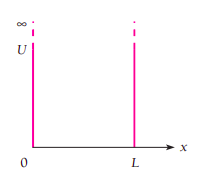
\includegraphics[width=6.5cm]{../../imagenes/pozo_potencial_infinito.png}
            \vspace{-0.5mm}
            \textbf{$Figura 1$} 
        \end{figure}
        
        \saltoPag

        \indent El movimiento de la partícula está restringido a la región $0 \leq x \leq L$ por paredes infinitamente altas ($U$ infinita). Una partícula no pierde energía al chocar con una pared infinitamente alta, por lo que la energía potencial de la partícula es infinita en los extremos de la caja, mientras $U$ es constante, diremos que $ U = 0 $ en el interior de la caja para conveniencia.Por que la partícula no puede tener una cantidad de energía potencial infinita, esta misma no puede existir fuera de la caja, por lo tanto $ \psi = 0$ para $x \leq 0$ y $x \geq L$, lo que tenemos que hacer es encontrar la función de onda $\psi$ para $0 < x < L$.\\
        \indent La ecuación de Schrödinger para una partícula en una caja es:

        \begin{align*}
            \frac{\partial^2 \psi}  {\partial x^2 }+ \frac{2m}{\hbar^2} (E - U) \psi = 0
        \end{align*}

        \indent Donde $U = 0$ en el interior de la caja. La solución general de esta ecuación es:

        \begin{align*}
            &\frac{\partial^2 \psi} {\partial x^2} + \frac{2m}{\hbar^2} \cdot E \cdot \psi = 0 \\
        \end{align*}

        \indent Para resolver esta ecuación, suponemos que $\psi = e^{r \cdot x}$, donde $r$ es una constante, entonces la derivada segunda de $\psi$ con respecto a $x$ es $\psi = r^2 \cdot e^{r \cdot x}$. Sustituyendo esto en la ecuación anterior, obtenemos:

        \begin{align*}
            &r^2 \cdot e^{r \cdot x} + \frac{2m}{\hbar^2} \cdot E \cdot e^{r \cdot x} = 0 \\
            &e^{r \cdot x} \cdot (r^2 + \frac{2m}{\hbar^2} \cdot E) = 0 \\
            &r^2 + \frac{2m}{\hbar^2} \cdot E = 0 \\
            &r^2 = -\frac{2m}{\hbar^2} \cdot E \\
            &r = \sqrt{-\frac{2m}{\hbar^2} \cdot E} \\
            &r = \pm j \cdot \frac{\sqrt{2mE}}{\hbar}\\
        \end{align*}

        \indent Entonces, la solución general de la ecuación de Schrödinger para una partícula en una caja es:

        \begin{align*}
            &\psi(x) =  C_1 \cdot e^{j \cdot \frac{\sqrt{2mE}}{\hbar} \cdot x} + C_2 \cdot e^{-j \cdot \frac{\sqrt{2mE}}{\hbar} \cdot x} \\
            &\psi(x) =  C_1 \cdot \cos(...) + j \cdot \sin(...) + C_2 \cdot\cos(...) - j \cdot \sin(...) \\
            &\psi(x) =  (C_1 + C_2) \cdot \cos(...) + j \cdot (C_1 - C_2) \cdot \sin(...) \\
            &\text{donde } j \cdot (C_1 - C_2) \text{ es una constante real que llamaremos } A, \\
            &\text{y } (C_1 + C_2) \text{ es otra constante que llamaremos } B
        \end{align*}

        \saltoPag
        \vspace{-10mm}

        \begin{align*}
            &\psi(x) = B \cdot \cos(\frac{\sqrt{2mE}}{\hbar} \cdot x) + A \cdot \sin(\frac{\sqrt{2mE}}{\hbar} \cdot x) \\
        \end{align*}
        \vspace{-5mm}

        \indent Las condiciones limites nos dicen que $\psi = 0$ en $x = 0$ y $x = L$. Si $cos (0) = 1$ ese termino no puede describir la función de onda, por lo que $B = 0$. Entonces, la función de onda para una partícula en una caja es:

        \begin{equation}
            \psi(x) = A \cdot \sin(\frac{\sqrt{2mE}}{\hbar} \cdot x)
        \end{equation}

        \indent En $x = L$ va a ser 0 para los valores de $E_n$:
        \vspace{-1mm}

        \begin{align*}
            &\frac{\sqrt{2mE}}{\hbar} \cdot L = n \cdot \pi \\
            &E = \frac{n^2 \cdot \pi^2 \cdot \hbar^2}{2m \cdot L^2}
        \end{align*}

        \indent Donde $n$ es un número cuántico, por lo tanto la energía de la partícula en una caja está cuantizada y ademas $E_n$ es un valor propio para cada $n$, si reemplazamos $E$ en la ecuación (2) obtenemos:

        \begin{align*}
            &\psi = A \cdot \sin(\sqrt{\frac{2mn^{2}\pi^{2\hbar^{2}}}{2mL^{2}}} \colon \hbar \cdot x)\\
            &\psi = A \cdot \sin(\frac{n\pi}{L} \cdot x)
        \end{align*}

        \indent Entonces obtemos la función propia para los valores propios $E_n$, esta función propia reuna todos los requerimientos necesarios, es decir, tiene un valor finito para cada número cuántico $n$, es univaluada en $x$ y $\psi$ y $\frac{\partial \psi}{\partial x}$ son continuas en $x = 0$ y $x = L$.

        \begin{equation}
            \psi_n = A \cdot sin(\frac{n\pi}{L} \cdot x)
        \end{equation}

        \indent Si calculamos $\left| \psi_n \right|^{2}$ sobre un espacio finito ($0 \leq x \leq L$) obtenemos:

        \begin{align*}
            &\int_{-\infty}^{\infty} \left| \psi_n \right|^{2} dx \\
            &\int_{0}^{L} \left| \psi_n \right|^{2} dx \\
            &\int_{0}^{L} A^{2} \cdot sin^{2}(\frac{n\pi}{L} \cdot x) dx \\
            &A^{2} \cdot \int_{0}^{L} sin^{2}(\frac{n\pi}{L} \cdot x) dx \\
            &A^{2} \cdot \int_{0}^{L} \frac{1 - cos(2 \cdot \frac{n\pi}{L} \cdot x)}{2} dx \\
            &A^{2} \cdot \int_{0}^{L} \frac{1}{2} - \frac{cos(2 \cdot \frac{n\pi}{L} \cdot x)}{2} dx \\
            &\frac{A^{2}}{2} \cdot \int_{0}^{L} 1 - \frac{cos(2 \cdot \frac{n\pi}{L} \cdot x)}{2} dx\\
        \end{align*}

        \saltoPag

        \vspace{-1mm}

        \begin{align*}
            &\frac{A^{2}}{2} \cdot \left[ x - \frac{L}{2n\pi} \cdot \sin(\frac{2nx\pi}{L}) \right]_{0}^{L} \\
            &\frac{A^{2}}{2} \cdot L = \int_{0}^{L} \left| \psi_n \right|^{2} dx \\
        \end{align*}

        \indent Para normalizar la función de onda, debemos hacer que $\int_{-\infty}^{\infty} \left| \psi_n \right|^{2} dx = 1$, por lo que $A^{2} \cdot L = 1$, entonces $A = \sqrt{\frac{2}{L}}$. Por lo tanto, la función de onda normalizada para una partícula en una caja/ pozo de potencial infinito es con condiciones limites $\psi(0) = \psi(L) = 0$:

        \begin{equation}
            \psi_n = \sqrt{\frac{2}{L}} \cdot sin(\frac{n\pi}{L} \cdot x)
        \end{equation}
    

        \section{Pozo de potencial finito}

            \subsection{Pozo de potencial finito simétrico}

            \indent La función de onda transpasa la pared con niveles de energía menores a la energía del pozo.

            \begin{figure}[h!]
                \centering
                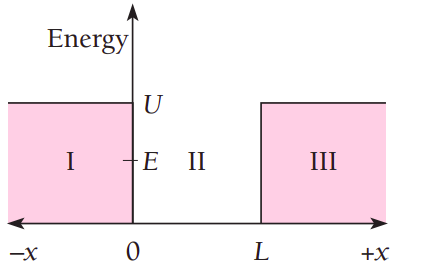
\includegraphics[width=6.5cm]{../../imagenes/pozo_potencial_finito.png}
                \vspace{-0.5mm}
                \textbf{$Figura 2$}
            \end{figure}

            \indent Tenemos un pozo de potencial de altura $U_0$ y ancho $L$. Si $E < U$, entonces la ecuación de Schrödinger es:

            \begin{align*}
                &\frac{\partial^2 \psi} {\partial x^2} + \frac{2m}{\hbar^2} \cdot (E - U) \cdot \psi = 0\\
                &\frac{\partial^2 \psi} {\partial x^2} - a^2 \cdot \psi = 0\\
            \end{align*}

            \indent Donde $a = \frac{\sqrt{2m(U - E)}}{\hbar}$, para resolver la ecuación diferencia tenemos que hacer la misma tecnica que en el pozo de potencial infinito, diciendo que:

            \begin{align*}
                &\psi = e^{r \cdot x} \\
                &\text{Su derivada segunda es} \\
                &\frac{\partial^2 \psi} {\partial x^2} = r^2 \cdot e^{r \cdot x} \\
            \end{align*}

            \indent Sustituyendo en la ecuación de Schrödinger obtenemos:

            \saltoPag

            \begin{align*}
                &r^2 \cdot e^{r \cdot x} - a^2 \cdot e^{r \cdot x} = 0 \\
                &e^{r \cdot x} \cdot (r^2 - a^2) = 0 \\
                &r^2 - a^2 = 0 \\
                &r^2 = a^2 \\
                &r = \pm a \\
            \end{align*}

            \indent Entonces, la solución general de la ecuación de Schrödinger para un pozo de potencial finito, en las regiones I y III es:

            \begin{align*}
                &\psi_I = C \cdot e^{a \cdot x} + D \cdot e^{-a \cdot x} \\ 
                &\psi_{III} = F \cdot e^{a \cdot x} + G \cdot e^{-a \cdot x} \\
            \end{align*}

            \indent Pero las solucines a las ecuación de Schrödinger deben ser finitas para que tengan sentido físico.\\
            \indent $\psi_I$  es la solucion para la región izquierda donde $x < 0$, si en esta region $x \rightarrow -\infty$ entonces $e^{-a \cdot x} \rightarrow \infty$, entonces D = 0.\\
            \indent Los mismo sucede para $\psi_{III}$, ya que esta es la solución para la región derecha donde $x > L$, si en esta region $x \rightarrow \infty$ entonces $e^{a \cdot x} \rightarrow \infty$, entonces F = 0, quedando como solución:\\

            \begin{equation}
                \psi_I = C \cdot e^{a \cdot x}
            \end{equation}

            \begin{equation}
                \psi_{III} = G \cdot e^{-a \cdot x} 
            \end{equation}

            \indent Para la región II, donde $0 < x < L$, la función de onda es $\psi_{II}$
            la partícula se encuentra en el pozo de potencial de altura finita, entonces la solucion es la misma a la primera parte del pozo de potencial infinito;\\

            \begin{equation}
                \psi_{II} = A \cdot sin(\frac{\sqrt{2mE}}{\hbar} \cdot x) + B \cdot cos(\frac{\sqrt{2mE}}{\hbar} \cdot x)
            \end{equation}

            \indent Para un potencial de pozo finito las condiciones limites eran $\psi(0) = \psi(L) = 0$, lo cual eliminaba al termino coseno, pero en este caso las condiciones son distitan, como la función de onda debe ser continua en $x = 0$ y $x = L$, entonces $\psi_I(0) = \psi_{II}(0)$ y $\psi_{II}(L) = \psi_{III}(L)$, por lo tanto, en $x = 0$: la función de onda $\psi_{II} = C$ y en $x = L$: la función de onda $\psi_{II} = G$

    \section{Efecto Túnel}

            \indent Una partícula sin la energía sufuciente para superar una barrera de potencial finita, puede atraversarla con el efecto túnel.\\

            \saltoPag

            \begin{figure}[h!]
                \centering
                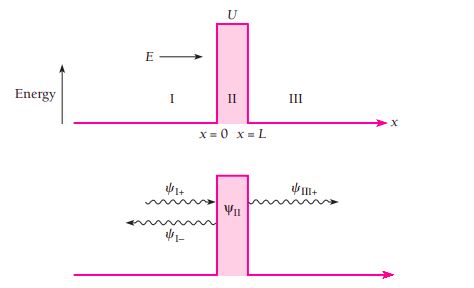
\includegraphics[width=7cm]{../../imagenes/efecto_tunel.png}
                \vspace{-0.5mm}
                \textbf{$Figura 3$}
            \end{figure}

            \indent En la figura 2, el pozo de potencial tenia una altura $U$ y una anchura $L$, pero la anchura de las regiones I y III es infinita, en este caso del efecto túnel, la región II tiene una anchura finita, en el caso del pozo con potencial finito las particulas efectivamente pasaban hacia las regiones I y III pero se quedaban atrapadas ahí.\\
            \indent Ahora vamos a imaginar la situación donde una partícula con energía $E < U$ se encuentra en la región I, donde la barrera es de altura $U$, cuando la particula choca con esta barrera tiene una psoibiblidad, pequeña pero no nula, de atravesarla y llegar a la región III, mientras más alta y más ancha sea la barrera, menos probable es que la partícula la atraviese.\\
            \indent EL efecto túnel es real, este ocurre por ejemplo con las partícuals alfa, donde una partícula cuya energía es de unos pocos MeV, mientras que el núcleo posee una barrera de potencial de unos 25 MeV, para que esto suceda la partícula tiene que chocar con la barrera aproximadamente $10^{38}$ veces o más,otr ejemplo son los diodos de tunel, donde la corriente eléctrica pasa a través de la barrera de potencial, en este caso la barrera es de unos pocos eV y la energía de los electrones es de unos pocos meV.\\
            \indent Vamos a considerar el caso de un conjunto idéntico, donde su energía es $E < U$, este conjunto incide desde la izquierda con una función de onda $\psi_{+I}$ donde esta representa al conjunto antes de chocar contra la pared, la función $\psi_{-I}$ a la parte del conjunto que se refleja, la función $\psi_{+III}$ represneta a la parte del conjunto que realizó efecto túnel y logró atravesar la barrera, finalmente la función $\psi_{-II}$ representa a la parte del conjunto que está atrapada dentro de la región II,dodne una parte hará el efecto túnel y la otra se reflejará.\\

            \indent La probabilidad de que una partícula atraviese la barrera de potencial es:

            \begin{equation}
                T = e^{-2 \cdot a \cdot L \cdot K_2}
            \end{equation}

            \indent Donde $K_2$ es:

            \begin{equation}
                K_2 = \frac{\sqrt{2m(U - E)}}{\hbar}
            \end{equation}
\end{document}
